\chapter{Diseño\label{sec:disenho}}

El diseño del dispositivo que se presenta en el proyecto tiene dos objetivos fundamentales. El primero de ellos es el de el sensado de la distancia entre las piernas del paciente donde se estudiaran los distintos tipos de sensores que permiten el cálculo, así como los dispositivos de procesado que existen en la actualidad para llevar a cabo la medida. El segundo de los objetivos es el de enviar la información de distancia desde el dispositivo hasta el PC donde se podrá realizar el procesado de los datos.

En el apartado \ref*{sec:fund_teóricos} se detallará cada una de las posibles tecnologías seleccionadas tanto para el sensado u obtención del dato de distancia como para el envío de los datos hasta el PC. Por último se determinará el prototipo final para la implementación del dispositivo. 

\section{Fundamentos teóricos}\label{sec:fund_teóricos}

 \subsection{Medida de distancia}
  \subsubsection{Radar}
  \subsubsection{Sensor de infrarrojos}
  \subsubsection{Sensor de ultrasonidos}
  
 \subsection{Tecnologías inalámbricas}
	 \subsubsection{802.11 (WiFi)}
	 \subsubsection{802.15 (Bluetooth)}
\section{Diseño final}

En la figura \ref{fig:esq_general} se observa un esquema general del diseño del prototipo del sistema.
\begin{figure}[htb]
	\centering
	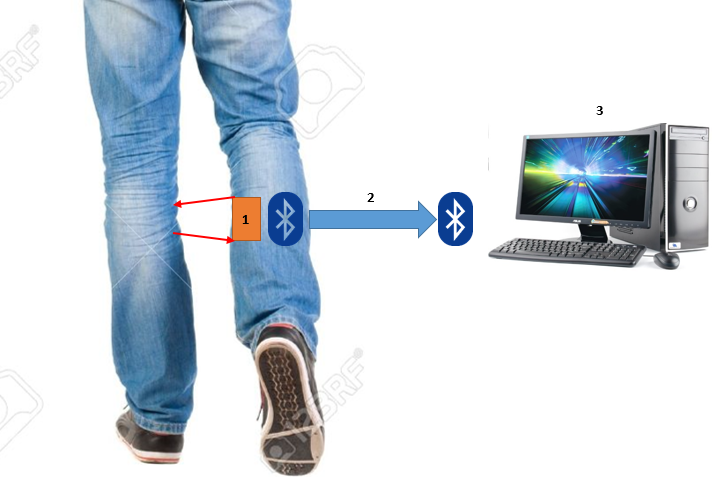
\includegraphics[width=0.8\textwidth]{./graphics/esq_general}
	\caption{Esquema general del sistema.} \label{fig:esq_general}
\end{figure}
